% Generated by code/needham.py -- do not edit by hand.
\definecolor{qocA}{rgb}{0.00,0.45,0.70}
\definecolor{qocB}{rgb}{0.90,0.60,0.00}
\definecolor{qocC}{rgb}{0.00,0.62,0.45}
\definecolor{qocD}{rgb}{0.80,0.40,0.00}
\definecolor{qocE}{rgb}{0.80,0.60,0.70}
\definecolor{qocF}{rgb}{0.35,0.70,0.90}
\begin{tikzpicture}[ink/.style={line width=0.9pt, ndInk}, faint/.style={line width=0.4pt, ndInk!35}, dashedink/.style={line width=0.5pt, ndInk!55, dash pattern=on 2.5pt off 2pt}, vec/.style={->, >=stealth, line width=1.2pt}, note/.style={font=\footnotesize\itshape, text=ndInk!85, align=center}, pointer/.style={->, >=stealth, line width=0.4pt, ndInk!60, shorten >=2pt, shorten <=1pt}, dot/.style={circle, fill=ndInk, inner sep=0pt, minimum size=3.4pt}, wash/.style={fill=ndSky, fill opacity=0.55}, every node/.style={text=ndInk}]
\definecolor{ndInk}{rgb}{0.13,0.13,0.18}
\definecolor{ndPaper}{rgb}{0.99,0.96,0.88}
\definecolor{ndSky}{rgb}{0.84,0.91,0.98}
\definecolor{ndRose}{rgb}{0.98,0.86,0.84}
\definecolor{ndBlue}{rgb}{0.13,0.36,0.66}
\definecolor{ndRed}{rgb}{0.78,0.20,0.16}
\definecolor{ndGold}{rgb}{0.88,0.62,0.10}
\definecolor{ndGreen}{rgb}{0.18,0.52,0.30}
\draw[faint, ->, >=stealth] (0.000,0.000) -- (6.864,0.000) node[right, text=ndInk] {shots $N$};
\draw[faint, ->, >=stealth] (0.000,0.000) -- (0.000,5.088) node[above, text=ndInk] {singular value};
\draw[faint] (0.000,0.060) -- (0.000,-0.060) node[below, font=\scriptsize, text=ndInk] {$10^{1}$};
\draw[faint] (1.320,0.060) -- (1.320,-0.060) node[below, font=\scriptsize, text=ndInk] {$10^{2}$};
\draw[faint] (2.640,0.060) -- (2.640,-0.060) node[below, font=\scriptsize, text=ndInk] {$10^{3}$};
\draw[faint] (3.960,0.060) -- (3.960,-0.060) node[below, font=\scriptsize, text=ndInk] {$10^{4}$};
\draw[faint] (5.280,0.060) -- (5.280,-0.060) node[below, font=\scriptsize, text=ndInk] {$10^{5}$};
\draw[faint] (6.600,0.060) -- (6.600,-0.060) node[below, font=\scriptsize, text=ndInk] {$10^{6}$};
\draw[faint] (0.060,0.640) -- (-0.060,0.640) node[left, font=\scriptsize, text=ndInk] {$10^{-2}$};
\draw[faint] (0.060,1.920) -- (-0.060,1.920) node[left, font=\scriptsize, text=ndInk] {$10^{-1}$};
\draw[faint] (0.060,3.200) -- (-0.060,3.200) node[left, font=\scriptsize, text=ndInk] {$10^{0}$};
\draw[faint] (0.060,4.480) -- (-0.060,4.480) node[left, font=\scriptsize, text=ndInk] {$10^{1}$};
\draw[line width=0.9pt, ndBlue] (0.000,4.344) -- (6.600,4.344);
\draw[line width=0.9pt, ndGold, dash pattern=on 3pt off 2pt] (0.000,4.280) -- (6.600,4.280);
\draw[line width=0.9pt, ndBlue] (0.000,3.446) -- (6.600,3.446);
\draw[line width=0.9pt, ndGold, dash pattern=on 3pt off 2pt] (0.000,3.483) -- (6.600,3.483);
\draw[line width=0.9pt, ndBlue] (0.000,3.411) -- (6.600,3.411);
\draw[line width=0.9pt, ndGold, dash pattern=on 3pt off 2pt] (0.000,2.728) -- (6.600,2.728);
\draw[line width=0.9pt, ndBlue] (0.000,2.899) -- (6.600,2.899);
\draw[line width=0.9pt, ndGold, dash pattern=on 3pt off 2pt] (0.000,2.416) -- (6.600,2.416);
\node[font=\scriptsize, text=ndBlue, anchor=west] at (6.626,2.899) {$\sigma_4$};
\node[font=\scriptsize, text=ndGold!80!ndInk, anchor=west] at (6.626,2.416) {$\sigma_4$};
\node[font=\scriptsize, text=ndBlue, anchor=west] at (6.626,4.344) {$\sigma_1$};
\draw[line width=1.1pt, ndRed] (0.000,3.600) -- (0.660,3.318) -- (1.320,3.018) -- (1.980,2.654) -- (2.640,2.354) -- (3.300,2.027) -- (3.960,1.703) -- (4.620,1.396) -- (5.280,1.106) -- (5.940,0.777) -- (6.600,0.461);
\fill[ndRed] (0.000,3.600) circle (1.4pt);
\fill[ndRed] (0.660,3.318) circle (1.4pt);
\fill[ndRed] (1.320,3.018) circle (1.4pt);
\fill[ndRed] (1.980,2.654) circle (1.4pt);
\fill[ndRed] (2.640,2.354) circle (1.4pt);
\fill[ndRed] (3.300,2.027) circle (1.4pt);
\fill[ndRed] (3.960,1.703) circle (1.4pt);
\fill[ndRed] (4.620,1.396) circle (1.4pt);
\fill[ndRed] (5.280,1.106) circle (1.4pt);
\fill[ndRed] (5.940,0.777) circle (1.4pt);
\fill[ndRed] (6.600,0.461) circle (1.4pt);
\draw[dashedink] (1.467,0.000) -- (1.467,2.899);
\node[dot, fill=ndBlue, minimum size=4.5pt] at (1.467,2.899) {};
\draw[dashedink] (2.463,0.000) -- (2.463,2.416);
\node[dot, fill=ndGold!80!ndInk, minimum size=4.5pt] at (2.463,2.416) {};
\node[note, anchor=north west, text=ndRed] (f) at (4.092,2.304) {the noise floor: the fifth singular\\ value, about $6.6/\sqrt N$};
\draw[pointer] (f.south west) to[bend right=20] (4.356,1.604);
\node[note, anchor=south] at (4.488,4.954) {solid: the tilted state $\vec x_0$;\ dashed: tilted by $15^\circ$ only};
\node[note, anchor=north] at (2.046,1.216) {the weakest mode rises\\ above the floor at\\ $N\approx130$ and $N\approx700$};
\node[font=\small] at (3.300,-0.900) {(a) the singular values of $\Hankel(0)$ and the noise};
\draw[faint, ->, >=stealth] (9.300,0.000) -- (15.748,0.000) node[right, text=ndInk] {shots $N$};
\draw[faint, ->, >=stealth] (9.300,0.000) -- (9.300,5.088) node[above, text=ndInk] {error of the pole};
\draw[faint] (10.109,0.060) -- (10.109,-0.060) node[below, font=\scriptsize, text=ndInk] {$10^{2}$};
\draw[faint] (11.457,0.060) -- (11.457,-0.060) node[below, font=\scriptsize, text=ndInk] {$10^{3}$};
\draw[faint] (12.804,0.060) -- (12.804,-0.060) node[below, font=\scriptsize, text=ndInk] {$10^{4}$};
\draw[faint] (14.152,0.060) -- (14.152,-0.060) node[below, font=\scriptsize, text=ndInk] {$10^{5}$};
\draw[faint] (15.500,0.060) -- (15.500,-0.060) node[below, font=\scriptsize, text=ndInk] {$10^{6}$};
\draw[faint] (9.360,0.457) -- (9.240,0.457) node[left, font=\scriptsize, text=ndInk] {$10^{-3}$};
\draw[faint] (9.360,1.600) -- (9.240,1.600) node[left, font=\scriptsize, text=ndInk] {$10^{-2}$};
\draw[faint] (9.360,2.743) -- (9.240,2.743) node[left, font=\scriptsize, text=ndInk] {$10^{-1}$};
\draw[faint] (9.360,3.886) -- (9.240,3.886) node[left, font=\scriptsize, text=ndInk] {$10^{0}$};
\fill[ndRose, fill opacity=0.5] (9.300,0.000) rectangle (10.259,4.800);
\node[font=\scriptsize, anchor=south] at (10.259,4.800) {$N^*$};
\draw[line width=1.1pt, ndRed] (9.404,4.642) -- (10.109,4.437) -- (10.752,3.703) -- (11.457,3.056) -- (12.100,2.658) -- (12.804,2.257) -- (13.447,1.968) -- (14.152,1.709) -- (14.795,1.395) -- (15.500,1.110);
\fill[ndRed] (9.404,4.642) circle (1.4pt);
\fill[ndRed] (10.109,4.437) circle (1.4pt);
\fill[ndRed] (10.752,3.703) circle (1.4pt);
\fill[ndRed] (11.457,3.056) circle (1.4pt);
\fill[ndRed] (12.100,2.658) circle (1.4pt);
\fill[ndRed] (12.804,2.257) circle (1.4pt);
\fill[ndRed] (13.447,1.968) circle (1.4pt);
\fill[ndRed] (14.152,1.709) circle (1.4pt);
\fill[ndRed] (14.795,1.395) circle (1.4pt);
\fill[ndRed] (15.500,1.110) circle (1.4pt);
\node[font=\scriptsize, text=ndRed, anchor=west] at (15.540,1.110) {$-\gamma_1$};
\draw[line width=1.1pt, ndBlue] (9.404,4.800) -- (10.109,4.678) -- (10.752,3.143) -- (11.457,2.606) -- (12.100,2.283) -- (12.804,1.936) -- (13.447,1.649) -- (14.152,1.374) -- (14.795,1.065) -- (15.500,0.756);
\fill[ndBlue] (9.404,4.800) circle (1.4pt);
\fill[ndBlue] (10.109,4.678) circle (1.4pt);
\fill[ndBlue] (10.752,3.143) circle (1.4pt);
\fill[ndBlue] (11.457,2.606) circle (1.4pt);
\fill[ndBlue] (12.100,2.283) circle (1.4pt);
\fill[ndBlue] (12.804,1.936) circle (1.4pt);
\fill[ndBlue] (13.447,1.649) circle (1.4pt);
\fill[ndBlue] (14.152,1.374) circle (1.4pt);
\fill[ndBlue] (14.795,1.065) circle (1.4pt);
\fill[ndBlue] (15.500,0.756) circle (1.4pt);
\node[font=\scriptsize, text=ndBlue, anchor=west] at (15.540,0.904) {$-\Gamma\pm\imath\omega$};
\draw[line width=1.1pt, ndInk!60] (9.404,2.674) -- (10.109,2.646) -- (10.752,2.520) -- (11.457,2.343) -- (12.100,2.095) -- (12.804,1.796) -- (13.447,1.575) -- (14.152,1.297) -- (14.795,1.011) -- (15.500,0.709);
\fill[ndInk!60] (9.404,2.674) circle (1.4pt);
\fill[ndInk!60] (10.109,2.646) circle (1.4pt);
\fill[ndInk!60] (10.752,2.520) circle (1.4pt);
\fill[ndInk!60] (11.457,2.343) circle (1.4pt);
\fill[ndInk!60] (12.100,2.095) circle (1.4pt);
\fill[ndInk!60] (12.804,1.796) circle (1.4pt);
\fill[ndInk!60] (13.447,1.575) circle (1.4pt);
\fill[ndInk!60] (14.152,1.297) circle (1.4pt);
\fill[ndInk!60] (14.795,1.011) circle (1.4pt);
\fill[ndInk!60] (15.500,0.709) circle (1.4pt);
\node[font=\scriptsize, text=ndInk!60, anchor=west] at (15.540,0.560) {$0$};
\draw[dashedink] (12.100,3.058) -- (15.500,1.616);
\node[note, anchor=south west] at (13.613,2.474) {slope $-\tfrac12$};
\node[note, anchor=north west] (l) at (10.513,1.257) {below $N^*$ the weakest\\ mode is lost in the noise,\\ and the estimates fail};
\draw[pointer] (l.west) to[bend left=20] (9.839,1.029);
\node[font=\small] at (12.804,-0.900) {(b) the error of the poles found by Ho--Kalman};
\end{tikzpicture}
